\documentclass[11pt]{article}
\usepackage[margin=1in]{geometry}
\usepackage{amsmath,amssymb,amsthm,booktabs,graphicx,hyperref,enumitem}
\newtheorem{theorem}{Theorem}
\newtheorem{proposition}{Proposition}
\newtheorem{lemma}{Lemma}
\newtheorem{corollary}{Corollary}
\theoremstyle{remark}\newtheorem{remark}{Remark}
\newcommand{\Z}{\mathbb{Z}}
\newcommand{\R}{\mathbb{R}}
\newcommand{\norm}[1]{\lVert #1\rVert_1}
\title{Exact sliding-window path signatures in a wrapping integer ring:\\ an overflow guard and interval queries}
\author{Matteo Pozza\thanks{Independent. \texttt{metapozza@proton.me}. Code: \url{https://github.com/metapozza/sigring}.}}
\date{October 2026}
\begin{document}
\maketitle
\begin{abstract}
The truncated path signature of the last $W$ increments of a stream is usually recomputed for every window or maintained in floating point by multiplying in the new increment and multiplying out the old one with an inverse. The latter is cheap but can be badly wrong after one very large increment, such as an overnight gap in a time coordinate. We keep the factorial-cleared signature state of integer increments in the ring $\Z/2^{B}$ ($B=64,128$). Because reduction modulo $2^B$ is a ring homomorphism and the update is a division-free polynomial with integer coefficients, the result equals the true integer state whenever that state fits, even if intermediates wrap. We prove a tight bound $|t_m|\le L^m$ (with $L$ the $\ell_1$ path length of the window) that yields a rigorous runtime certificate, show that the group inverse of a signature is its antipode so that the signature of any interval of a stored stream is obtained exactly from two prefix states, and report tests of the claims, a determinism study across eight instruction sets, and benchmarks. The update kernel itself is not new; the contribution is the exact integer formulation, the guard, and an honest measurement of where it does and does not pay off. Speed is roughly equal to the best floating-point fused update and faster than recomputation. An implementation (Rust crate and Python wheel) is available under a source-available licence.
\end{abstract}

\section{Introduction}
The signature of a path is the sequence of its iterated integrals and is a standard feature map for sequential data \cite{chen1958,lyons1998}; for financial streams see \cite{gyurko2013}. For a stream of $d$-dimensional increments one often needs the truncated signature (depth $N$) of the most recent $W$ increments at every tick. Two natural approaches are (i) recompute each window, costing $O(W\,d^N)$ per tick up to constants, and (ii) maintain the state $S$ and update $S'=E(-x_{\mathrm{old}})\otimes S\otimes E(x_{\mathrm{new}})$, costing $O(d^N)$ per tick independent of $W$, where $E$ is the tensor exponential. In floating point (ii) is numerically fragile: after a huge increment enters and later leaves the window, rounding errors committed at the scale of that increment persist at the scale of the (much smaller) true values.

We observe that for integer increments everything can be done exactly in $\Z/2^B$, and we state and test the consequences. We make no claim about trading performance; this is a feature-extraction primitive.

\paragraph{Contributions.} (1) An exact, division-free, allocation-free sliding update in $\Z/2^{B}$ (Section~\ref{sec:update}). (2) A tight bound $|t_m|\le L^m$ and the resulting runtime certificate (Section~\ref{sec:guard}). (3) Exact interval queries via the antipode (Section~\ref{sec:interval}). (4) Tests, a cross-architecture determinism study, and benchmarks with explicit caveats (Section~\ref{sec:exp}).

\paragraph{What is not new.} The Horner-style fused multiply-exponentiate kernel is that of Signatory \cite{kidger2021}, which also supports interval queries from stored prefix signatures and a float inverse. Sliding-window aggregation of associative operators is a studied problem \cite{tangwongsan2017}; the signature is a monoid, so a two-stack scheme applies and is our float baseline. Our contribution is the exact integer formulation and its guarantees.

\section{Setting}
Let $x_1,\dots,x_W\in\Z^d$ be integer increments (real data are quantised: price $\to$ ticks, time $\to$ milliseconds; a scale $K$ converts back, $S_n^{\mathrm{real}}=S_n/K^n$). For $x\in\R^d$ let $E(x)=\sum_{n\ge0}x^{\otimes n}/n!$ in the truncated tensor algebra $T^{\le N}(\R^d)$. The signature of the piecewise-linear path through the increments is $S=E(x_1)\otimes\cdots\otimes E(x_W)$ (Chen). Write $S=(1,S_1,\dots,S_N)$ with $S_n\in(\R^d)^{\otimes n}$. The \emph{scaled state} is $t_n=n!\,S_n$.

\begin{lemma}\label{lem:int}
$t_n\in(\Z^d)^{\otimes n}$ for integer increments. Moreover scaled tensors multiply by $(A\cdot B)_m=\sum_{k=0}^m\binom mk A_k\otimes B_{m-k}$ (with $A_0=B_0=1$), and the scaled exponential of $x$ is $E(x)_n=x^{\otimes n}$.
\end{lemma}
\begin{proof}
Expanding the product, $S_n=\sum_{n_1+\dots+n_W=n}\prod_i x_i^{\otimes n_i}/n_i!$ (ordered tensor products), so $t_n=\sum\binom{n}{n_1,\dots,n_W}\bigotimes_i x_i^{\otimes n_i}$ with integer multinomial coefficients. For the product rule, $m!\,(A^S\!\otimes B^S)_m=\sum_k \frac{m!}{k!(m-k)!}(k!A^S_k)\otimes((m-k)!B^S_{m-k})$. The last statement is $n!\,x^{\otimes n}/n!$.
\end{proof}

\section{The exact sliding update}\label{sec:update}
Since $S=E(x_{\mathrm{old}})\otimes S_{\mathrm{rest}}$ for the oldest increment, the window slides by $S'=E(-x_{\mathrm{old}})\otimes S\otimes E(x_{\mathrm{new}})$. By Lemma~\ref{lem:int} this is a polynomial in the entries of $t$ and the increments with integer coefficients (binomials). A division-free Horner form computes, for each level $m$ (descending, so lower levels are still old values), $M_0=1$, $M_j=M_{j-1}\otimes r+\binom mj t_j$ and $t'_m=M_m$ for a right push of $r$, and the mirror form $M_j=l\otimes M_{j-1}+\binom mj t_j$ for the left multiplication by $l=-x_{\mathrm{old}}$. This costs a small constant times $N\,d^N$ multiplications and no division.

\begin{proposition}[Exactness]\label{prop:exact}
Let $\pi:\Z\to\Z/2^B$ be reduction. Computing the update in $\Z/2^B$ yields $\pi(t')$, where $t'$ is the true integer state. Hence if every entry of $t'$ lies in $[-2^{B-1},2^{B-1})$, its centered lift is recovered exactly, even if intermediate values wrapped.
\end{proposition}
\begin{proof}
$\pi$ is a ring homomorphism and the update is an integer polynomial.
\end{proof}

\section{A tight overflow guard}\label{sec:guard}
Let $\norm{\cdot}$ be the sum of absolute values of tensor entries. It is multiplicative: $\norm{a\otimes b}=\norm a\norm b$.

\begin{theorem}\label{thm:guard}
Let $L=\sum_{i=1}^W\norm{x_i}$. Then $\norm{t_m}\le L^m$ for all $m$; in particular every entry satisfies $|t_m|\le L^m$. The bound is attained.
\end{theorem}
\begin{proof}
By multiplicativity, $\norm{S_m}\le\sum_{n_1+\dots+n_W=m}\prod_i\norm{x_i}^{n_i}/n_i!=[z^m]\prod_i e^{\norm{x_i}z}=L^m/m!$. Multiply by $m!$. For $d=1$ and all $x_i\ge0$, $S_m=(\sum x_i)^m/m!$ so $t_m=L^m$.
\end{proof}
\begin{corollary}[Certificate]
If $L^N<2^{B-1}$ (and $L\ge1$) then all levels $m\le N$ fit, so by Proposition~\ref{prop:exact} the ring state equals the true state. $L$ is maintained exactly as a sliding sum of integers.
\end{corollary}
The largest certifiable $L$ is $2^{(B-1)/N}$: for $N=3$, $2.1\times10^6$ ($B=64$) and $5.5\times10^{12}$ ($B=128$); for $N=4$, $5.5\times10^4$ and $3.6\times10^9$. The certificate is sufficient, not necessary: it can refuse a window whose true state happens to fit.

\section{Exact interval queries via the antipode}\label{sec:interval}
\begin{proposition}\label{prop:anti}
The group inverse of the signature $S_{(x_1..x_k)}$ is $S_{(-x_k,\dots,-x_1)}$, whose level-$n$ component is $(-1)^n$ times the index-reversal of $S_n$; the same holds for scaled states. Consequently, for prefix states $P_i$ (increments $1..i$), the state of increments $i{+}1..j$ is $P_i^{-1}\cdot P_j$ in the scaled product.
\end{proposition}
\begin{proof}
$E(-x)\otimes E(x)=1$, so $E(-x_k)\otimes\cdots\otimes E(-x_1)$ inverts $E(x_1)\otimes\cdots\otimes E(x_k)$; reversing the order of tensor factors and negating gives the stated formula. The scaling $n!$ is symmetric.
\end{proof}
Storing prefix states and applying the antipode (free: a permutation and sign flip) gives any interval exactly in the ring, with no float inverse. By Proposition~\ref{prop:exact} the prefixes themselves may have wrapped: the result equals the interval's true state mod $2^B$, exact whenever the \emph{interval's} guard $L_{[i,j)}^N<2^{B-1}$ holds. (Signatory warns of instability for large intervals when using a float inverse \cite{kidger2021}; in a small test we did not observe large float error, so our claim concerns guarantees, not a demonstrated failure of that method.)

\section{Experiments}\label{sec:exp}
All timings are from a single 2-core 2.1\,GHz Xeon sandbox with about $\pm25\%$ run-to-run noise; they indicate orders of magnitude, not tight constants.

\paragraph{Correctness tests.} The state equals recomputation from scratch for $i64$ and $i128$ over randomised streams and shapes; the Horner and a reference power-tensor kernel are bit-identical; interval queries equal direct recomputation, including when the stored prefixes overflowed $i64$; and Theorem~\ref{thm:guard} was checked on 32{,}400 (window, level) pairs with no violation, equality attained 6{,}613 times. Log-signature coordinates (Lyndon words and brackets) agree with pySigLib to $6\times10^{-16}$ and with signature-rs to $1.6\times10^{-15}$.

\paragraph{Where the float fused update fails.} For $d=2$, $N=4$, $W=64$: scale-relative error of the float fused update against the exact state was $1.7\times10^{-11}$ on a random walk, $8.1\times10^{-6}$ on heavy-tailed increments and $0.56$ on a stream with spikes. On a public sample of real E-mini S\&P~500 ticks, with path (price, time) and a 6.5-hour gap, the float fused update had scale-relative error (worst entry error divided by the largest exact entry) of $4.3\times10^{9}$, i.e.\ garbage, while the 128-bit ring matched an exact oracle; the same stream with a (price, volume, time) path gave $0.83$, and for hourly and daily bars the float error was $10^{-13}$--$10^{-12}$. Figure~\ref{fig:gap} isolates the mechanism on synthetic ticks (price $\pm3$ ticks, 50--150\,ms between ticks, a 6.5-hour gap every 20{,}000 ticks): once the first gap has passed, the float fused state has relative error of order one for the rest of the run, whereas a float \emph{recompute} of the same window agrees with the ring exactly and the 128-bit guard certifies all 199{,}937 windows (64-bit certifies 199{,}361, refusing exactly those containing a gap).
\begin{figure}[t]\centering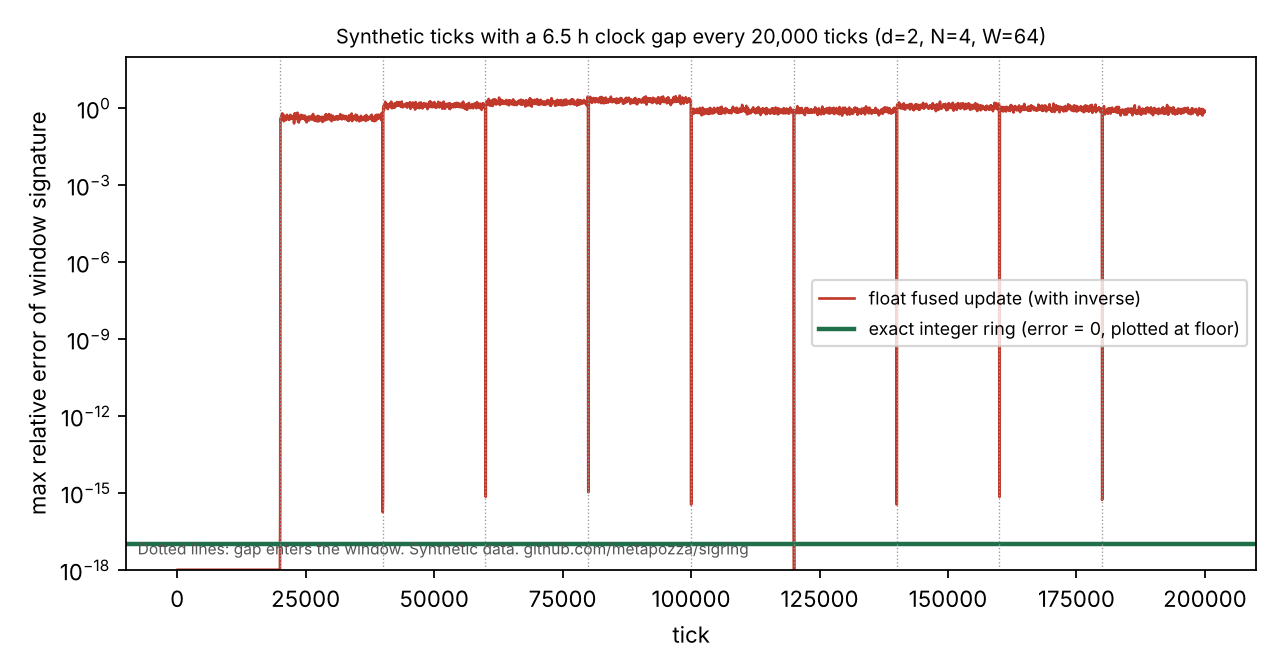
\includegraphics[width=0.85\linewidth]{fig_gap.png}
\caption{Synthetic stream with a clock gap every 20{,}000 ticks. The exact ring has zero error; the float fused update does not recover after the first gap leaves the window.}\label{fig:gap}\end{figure}

\paragraph{Performance.} Nanoseconds per tick (one push and one pop), Horner kernels for all methods:
\begin{center}\small\begin{tabular}{lrrrr}\toprule
$(d,N,W)$ & ring $i64$ & ring $i128$ & float fused & float two-stack\\\midrule
(2,4,64) & 329 & 442 & 233 & 427\\
(3,4,64) & 511 & 1151 & 436 & 743\\
(5,3,64) & 382 & 958 & 386 & 651\\
(2,4,256) & 220 & 386 & 175 & 394\\\bottomrule\end{tabular}\end{center}
Repeated runs at $(2,4,64)$ gave $i64$ 221--299\,ns against 213--286\,ns for the float fused update: a tie within noise. Against recomputing every window with pySigLib ($d=2$, $N=4$), the ring was about 4--5$\times$ faster at $W=64$, 12$\times$ at $W=256$, 47$\times$ at $W=1024$ and at parity at $W=16$. On real hourly EURUSD (4{,}832 windows, $d=15$, $N=3$, 336 increments) one window cost 39\,$\mu$s ($i64$), 71\,$\mu$s ($i128$), 243\,$\mu$s (pySigLib) and 3{,}326\,$\mu$s (iisignature), with agreement to $1.5\times10^{-16}$ against iisignature. State memory was about 69\,KB against 9.7\,MB for a float two-stack, whose per-push 99.9th percentile was 4.6\,ms against 55\,$\mu$s for the ring at that shape.

\paragraph{Determinism.} State hashes were identical across eight Rust build variants and an independent C port on x86-64 (gcc, clang), aarch64, riscv64, ppc64 (big-endian), s390x (big-endian), arm32, mips32 (big-endian, 64-bit state only) and wasm32. A plain-float Rust build was also bit-identical across six x86-64 variants, so the practical advantage is for C/C++ code (a C float control split into two bit patterns under FMA contraction), threaded or GPU reductions, and cross-architecture reproducibility.

\paragraph{Guard on real data.} The 128-bit guard certified 100\% of windows on every real dataset tried (E-mini ticks, EURUSD hourly, daily equities, index bars). The 64-bit guard depends on units: it passes at coarse units and fails at depth 4 with cent or $10^{-5}$ units.

\section{Limitations}
Increments must be integers after scaling; units and depth bound the usable resolution. Cost grows as $d^N$; there is no sparse or Lyndon-basis internal state and no autodiff or GPU path. The float fused update is as fast, and for well-scaled data is accurate; the benefit of the ring is exactness, reproducibility and the certificate. Benchmarks are from one noisy machine. We did not test embedded targets, DABA-style baselines, or live market feeds, and we make no claim about predictive value.

\section*{Availability}
Rust crate \texttt{sigring} and Python package \texttt{sigring}; source at \url{https://github.com/metapozza/sigring} under the PolyForm Noncommercial License 1.0.0 (free for personal, research, educational and non-profit use; commercial use by agreement). Tests, determinism hashes and benchmark harnesses are in the repository.

\begin{thebibliography}{9}
\bibitem{chen1958} K.-T. Chen. Integration of paths---a faithful representation of paths by noncommutative formal power series. \emph{Trans. Amer. Math. Soc.} 89 (1958).
\bibitem{lyons1998} T. Lyons. Differential equations driven by rough signals. \emph{Rev. Mat. Iberoamericana} 14 (1998).
\bibitem{gyurko2013} L.~G. Gyurk\'o, T. Lyons, M. Kontkowski, J. Field. Extracting information from the signature of a financial data stream. arXiv:1307.7244.
\bibitem{kidger2021} P. Kidger, T. Lyons. Signatory: differentiable computations of the signature and logsignature transforms, on both CPU and GPU. \emph{ICLR} 2021 (arXiv:2001.00706).
\bibitem{tangwongsan2017} K. Tangwongsan, M. Hirzel, S. Schneider. Low-latency sliding-window aggregation in worst-case constant time. \emph{DEBS} 2017.
\end{thebibliography}
\end{document}
